\chapter{Instrumentation}

Dazu wurde ein Tracer implementiert, durch welchem die 
Channel- und Lock-Operationen, sowie andere Operationen wie Select und das 
erzeugen einer neuen Routine, ersetzt, bzw. erweitert werden. Diese 
führen die eigentlichen Operationen aus und zeichnen gleichzeitig den 
Trace auf. Die Ersetzung durch die Drop-In Replacements kann dabei automatisch 
durch einen Instrumenter erfolgen, welche mit Hilfe des Abstract Syntax Tress 
die Ersetzungen vornimmt.\\
Anders als in vielen anderen Programmen, welche den Trace von Go-Programmen
analysieren, wie z.B.~\cite{GoAt2} oder~\cite{GoVis} wird dabei der Tracer 
selbst implementiert und basiert nicht auf dem Go-Runtime-Tracer~\cite{GoRunTrace}. 
Dies ermöglicht es, den Tracer genau auf die benötigten Informationen zuzuschneiden
und so einen geringeren negativen Einfluss auf die Laufzeit des Programms zu erreichen.\\\\
Der Aufbau des Trace basiert auf~\cite{PPDP18}. Er wird aber um Informationen 
über Locks erweitert. Der Trace wird für jede Routine
separat aufgezeichnet. Außerdem wird, anders als in~\cite{PPDP18} ein globaler
Program-Counter für alle Routinen und nicht ein separater Counter für jede 
Routine verwendet. Dies ermöglicht es bessere Rückschlüsse über den genauen 
Ablauf des Programms zu ziehen.
\todo{umschreiben}

\section{Trace}

Um diesen Trace zu erzeugen, werden die Standartoperation aud Go durch Elemente
des Tracers ersetzt. Die Funktionsweisen dieser Ersetzungen sind im folgenden 
angegeben. Dabei werden nur solche Ersetzungen angegeben, welche direkt 
für die Erzeugung
des Traces notwendig sind. Zusätzlich werden noch 
weitere Ersetzungen durchgeführt, wie z.B. die Ersetzung der Erzeugung von 
Mutexen und Channel von den Standardvarianten zu den Varianten des Tracers.
Hierbei wird auch die Größe jedes Channels gespeichert.
Dies werden in der Übersicht zur Vereinfachung nicht betrachte. Auch werden 
in der Übersicht nur die Elemente betrachtet, die für die Durchführung der 
Operation und dem Aufbau des Traces benötigt werden. Hilfselemente, wie z.B. 
Mutexe, welche verhindern, dass mehrere Routinen gleichzeitig auf die selbe 
Datenstruktur, 
z.B. die Liste der Listen, welche die Traces für die einzelnen Routinen 
speichern, zugreifen, werden nicht mit angegeben. Dabei sei $c$ ein 
Zähler, $nR$ ein Zähler für die Anzahl der Routinen, $nM$ ein Zähler für die 
Anzahl der Mutexe und $nC$ ein Zähler für die Anzahl der Channels. $nM$ und $nC$
werden bei der Erzeugung eines neuen Mutex bzw. eines neuen Channels atomarisch 
Incrementiert. Den erzeugten Elementen wird er neue Wert als $id$ zugeordnet. All diese 
Zähler seien global und zu Beginn als $0$ initialisiert. Außerdem bezeichnet 
$mu$ einen Mutex, $rmu$ einen RW-Mutex, $ch$ einen Channel und $B$ bzw. $B_i$
mit $i\in\mathbb{N}$ den 
Körper einer Operation. Zusätzlich
sei $id$ die $Id$ der Routine, in der eine Operation ausgeführt wird,
$[signal(t, i)]^{id}$ bedeute, dass der das entsprechende Element (hier als 
Beispiel $signal(t, i))$, in den Trace der Routine mit id $id$ eingeführt wird
und $[+]^i$ bedeute, das in die Liste der Traces ein neuer, leerer Trace 
eingefügt wird, welcher für die Speicherung des Traces der Routine $i$ 
verwendet wird. 
$\langle a|b\rangle$ bedeutet, dass ein Wert je nach Situation auf $a$ oder $b$ gesetzt 
wird. Welcher Wert dabei verwendet wird, ist aus der obigen Beschreibung der 
Trace-Elemente erkennbar. $\text{e}_1$ bis $\text{e}_n$ bezeichnet die Selektoren in einem Select statement.
$\text{e}_i^*$ bezeichnet dabei einen Identifier für einen Selektor, der sowohl die 
Id des beteiligten Channels beinhaltet, als auch die Information, ob es sich um ein 
Send oder Receive handelt und $\text{e}_i^m$ die Message, die in einem Case 
empfangen wurde. 
\begin{tabular}{lcl}
  go B & $\Rightarrow$ & nr := atomicInc(nR); ts := atomicInc(c); [ signal(ts, nr) ]$^\text{nr}$;\\
    & & [+]$^\text{nr}$; go \{ ts' := atomicInc(c); [ wait(ts, nr) ]$^\text{id}$; B\};\\
  ch <- i & $\Rightarrow$ & ts := atomicInc(c); [ pre(ts, ch.id, true) ]$^\text{id}$; ch <- \{i, id, ts\};\\
    & & ts' := atomicInc(c); [ post(ts', ch.id, true, id) ]$^\text{id}$\\
  <- ch & $\Rightarrow$ & ts := atomicInc(c); [ pre(ts, ch.id, false) ]$^\text{id}$;\\
    & & \{i, id\_send, ts\_send\} := <-c; ts' := atomicInc(c);\\
    & & [ post(ts', ch.id, false, id\_send, ts\_send) ]$^\text{id}$; return i;\\
  % close(ch) & $\Rightarrow$ & ts := atomicInc(c); close(ch); [ close(ts, ch.id) ]$^\text{id}$\\
  select(e$_\text{i} \leadsto \text{B}_\text{i}$) & $\Rightarrow$ & ts := atomicInc(c); [ pre(ts, e$_1^*$, $\ldots$, e$_n^*$, false) ]$^\text{id}$;\\
    & & select(e$_\text{i} \leadsto$ \{ ts' := atomicInc(c);\\
    & & [ $\langle \text{post(ts, e$_\text{i}$.ch, false, e$_\text{i}^\text{m}$.id\_send, e$_\text{i}^\text{m}$.ts\_send)}\ |$ \\
    & & post(ts, e$_\text{i}$.ch, true, id) $\rangle$ ]$^\text{id}$ B$_\text{i}$\}) \\
  select(e$_\text{i} \leadsto \text{B}_\text{i}$ | B$_\text{def}$) & $\Rightarrow$ & ts := atomicInc(c); [ pre(ts, e$_1^*$, $\ldots$, e$_n^*$, false) ]$^\text{id}$;\\
    & & select(e$_\text{i} \leadsto$ \{ ts' := atomicInc(c);\\
    & & [ $\langle \text{post(ts, e$_\text{i}$.ch, false, e$_\text{i}^\text{m}$.id\_send, e$_\text{i}^\text{m}$.ts\_send)}\ |$ \\
    & & post(ts, e$_\text{i}$.ch, true, id) $\rangle$ ]$^\text{id}$ B$_\text{i}$\} |\\
    & & ts' := atomicInc(c); [ default(ts) ]$^\text{id}$; B$_\text{def}$) \\
  mu.(Try)Lock() & $\Rightarrow$ & ts := atomicInc(c); mu.(Try)Lock();\\
    & & [ lock(ts, mu.id, $\langle \text{-|t}\rangle$, $\langle \text{0|1}\rangle$) ]$^\text{id}$;\\
  mu.Unlock() & $\Rightarrow$ & ts := atomicInc(c); mu.Unlock(); [ unlock(ts, mu.id) ]$^\text{id}$;\\
  rmu.(Try)(R)Lock() & $\Rightarrow$ & ts := atomicInc(c); rmu.(Try)(R)Lock();\\
    & & [ lock(ts, rmu.id, $\langle \text{-|t|r|tr}\rangle$, $\langle \text{0|1}\rangle$) ]$^\text{id}$;\\
  rmu.Unlock() & $\Rightarrow$ & ts := atomicInc(c); rmu.Unlock(); [ unlock(ts, rmu.id) ]$^\text{id}$;
\end{tabular}
\todo{Mehr}

\section{Select}\label{Chap:Inst-Sec:Select}
Ein Beispiel dazu findet sich 
in Abb.~\ref{Chap:Analyze-Sec:Channel-SubSec:Select-Fig:GFuzz_Inst}.
\begin{figure}[h!]
  \begin{minipage}[t]{0.3\textwidth}
    \lstinputlisting[xrightmargin=-50pt]{code/gfuzz-select-pre.txt}
  \end{minipage}
  \begin{minipage}[t]{0.65\textwidth}
    \lstinputlisting[xrightmargin=40pt]{code/gfuzz-select-post.txt}
  \end{minipage}
  \caption{Beispiel für die Order-Enforcement-Instrumentierung eines Select-Statements 
  durch GFuzz for (links) und nach der Implementierung (rechts). Ersetze $......$
  in dem Programm nach der Instrumentierung (rechts) durch das Programm vor der 
  Instrumentierung (links).~\cite[gekürzt]{gfuzz}}
  \label{Chap:Analyze-Sec:Channel-SubSec:Select-Fig:GFuzz_Inst}
\end{figure}








\todo{Abschnitt einfügen}
\section{Instrumenter}\label{Chap:Tracer-Sec:Instrumenter}
\draft{Instrumenter}
Um den Trace zu erzeugen, müssen verschiedene Operationen durch Funktionen
des Tracers ersetzt bzw. erweitert werden. Wie man an dem Beispiel 
unschwer erkennen kann, besitzt die Version mit dem Tracer einen deutlich längeren
Programmcode, was bei der Implementierung zu einer größeren Arbeitslast 
führen kann. Da sich der Tracer auch negativ auf die Laufzeit des Programms 
auswirken kann, ist es in vielen Situationen nicht erwünscht, ihn in den 
eigentlichen Release-Code einzubauen, sondern eher in eine eigenständige 
Implementierung, welche nur für den Tracer verwendet werden. Um dies zu
automatisieren wurde ein zusätzliches Programm implementiert, welches in der 
Lage ist, den Tracer in normalen Go-Code einzufügen. Die Implementierung, 
welche ebenfalls in~\cite{GoChan} zur Verfügung steht, arbeitet mit einem 
Abstract Syntax Tree. Bei dem Durchlaufen dieses Baums werden die 
entsprechenden Operationen in dem Programm erkannt, und durch ihre entsprechenden 
Tracer-Funktionen ersetzt bzw.\ ergänzt. Neben dem Ersetzen der verschiedenen 
Operationen werden außerdem einige Funktionen hinzugefügt. Zu Begin der 
Main-Funktion des Programms wird der Tracer initialisiert. Zusätzlich
wird eine zusätzliche Go-Routine gestartet, in welcher ein Timer läuft. 
Ist dieser abgelaufen, wird  die Analyse gestartet, 
auch wenn das Programm noch nicht vollständig durchlaufen ist. Dies führt dazu,
dass auch Programme, in welchen ein Deadlock aufgetreten ist, analysiert 
werden können. Endet das Programm in der vorgegebenen Zeit, wird der Analyzer 
nach der Beendigung des Programms gestartet.

\extend{Instrumenter}

\section{Laufzeit}\label{Chap:Tracer-Sec:Laufzeit}
\paragraph{Instrumenter} Zuerst soll die Laufzeit des Instrumenters betrachtet 
werden. Es ist erwartbar, 
dass sich die Laufzeit linear in der Anzahl der Ersetzungen in dem AST, also 
der Anzahl der Mutex- und Channel-Operationen verhält. Dies bestätigt sich auch durch 
die Messung der Laufzeit des Programms (vgl. 
Abb.~\ref{Chap:Tracer-Sec:Laufzeit-Img:LaufzeitInstrumenter})\\
\begin{minipage}{0.45\textwidth}
  \centering  
  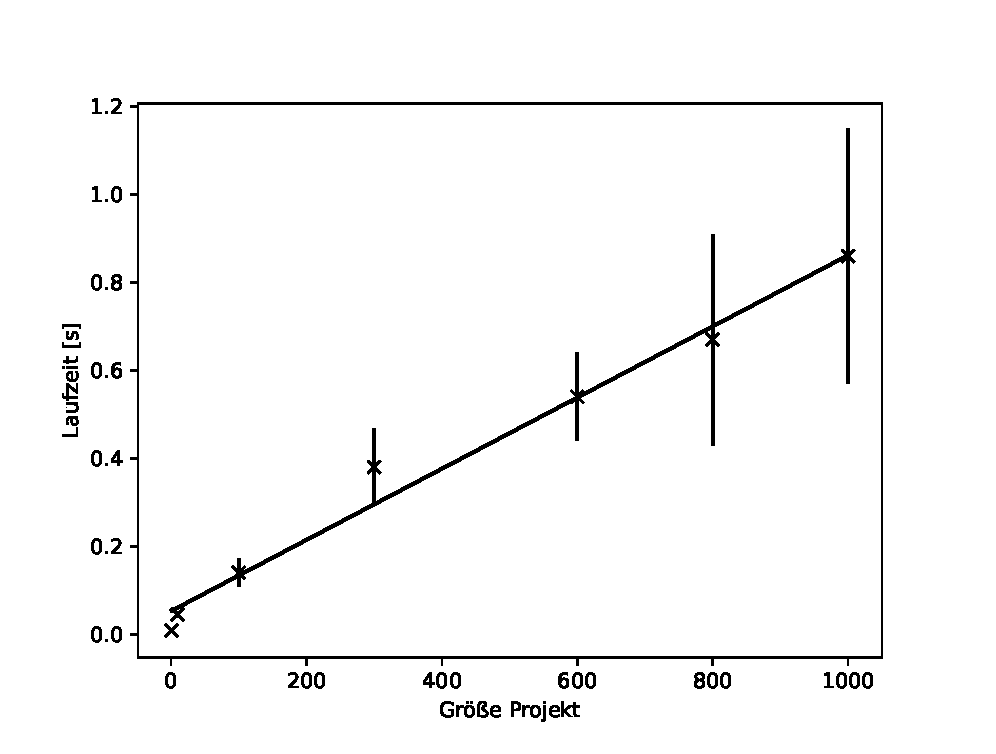
\includegraphics[width=\textwidth]{img/Runtime_Instrumenter.eps}
  \captionof{figure}{Laufzeit des Instrumenters}
  \label{Chap:Tracer-Sec:Laufzeit-Img:LaufzeitInstrumenter}
\end{minipage}
\hfill
\begin{minipage}{0.45\textwidth}
  \centering
  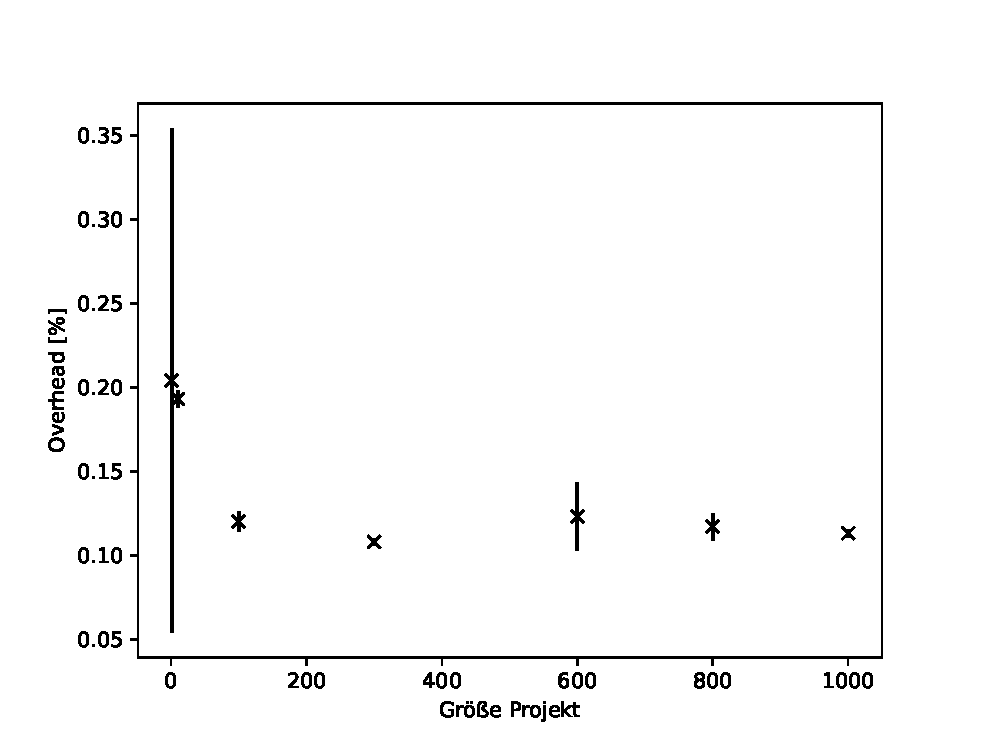
\includegraphics[width=\textwidth]{img/Runtime_Tracer.eps}
  \captionof{figure}{Prozentualer Overhead des Tracers ohne Analyse}
  \label{Chap:Trace-Sec:Laufzeit-Img:LaufzeitTracer}
\end{minipage}
Der abgebildete Graph zeigt die Laufzeit des Programms in $s$ abhängig von der 
Größe des Programms. Das Programm besteht dabei aus einem Testprogramm, welches 
alle möglichen Situationen mit Channels und Mutexen abbildet. Die Vergrößerung 
des Programmes wurde dadurch erreicht, dass die Datei mit dem Programmcode 
mehrfach in dem Projekt vorkam. Ein Projekt mit Größe $n$ besteht vor der 
Instrumentierung also 
aus $n$ Dateien, mit insgesamt $65n$ Zeilen von Code und $52n$ Ersetzungen
in dem AST. Die tatsächliche Laufzeit des Instrumenters auf einen 
Programm hängt schlussendlich natürlich von der tatsächlichen Größe des 
Projekt und der Verteilung der Mutex- und Channel-Operationen in dem Code ab.\\
\begin{table}[!h]
  \centering
  \begin{tabular}{|c|c|c|c|c|}
  \hline
  Projekt & LOC & Nr. Dateien & Nr. Ersetzungen & Zeit {[}s{]} \\ \hline
  ht-cat & $733$ & $7$ & $233$ & $0.013 \pm 0.006$ \\ \hline
  go-dsp & $2229$ & $18$ & $600$ & $0.029 \pm 0.009$ \\ \hline
  goker & $9783$ & $103$ & $4928$ & $0.09 \pm 0.03$ \\ \hline
  \end{tabular}
  \caption{Laufzeit des Instrumenters für ausgewählte Programme}
  \label{Chap:Tracer-Sec:Laufzeit-Tab:LaufzeitInstrumenter}
\end{table}
Zusätzlich wurde die Messung auch mit drei tatsächlichen Programmen 
durchgeführt. Die dort gemessenen Werte befinden sich in 
Tabelle~\ref{Chap:Tracer-Sec:Laufzeit-Tab:LaufzeitInstrumenter}. Gerade in 
Abhängigkeit von der Anzahl der Ersetzungen, stimmen die hier gemessenen Werte
mit denen in Abb.~\ref{Chap:Tracer-Sec:Laufzeit-Img:LaufzeitInstrumenter} gut 
überein, während es bei den anderen Parametern größere Abweichungen gibt.
Dies bestätigt dass der dominante Faktor für die Laufzeit des Programms 
die Anzahl der Ersetzungen in dem AST ist, und die Laufzeit linear von dieser 
abhängt.
\paragraph{Tracer} Folgend soll nun auch die Laufzeit des Tracers betrachtet werden.
Hierbei wird nur die Laufzeit des eigentlichen Tracers, nicht aber der anschließenden 
Analyse betrachtet. Um den Overhead in Abhängigkeit von der Größe des Projektes messen 
zu können, wird das selbe Testprogramm betrachtet, welches bereits in der Messung 
für den Instrumenter verwendet wurde. Abb. \ref{Chap:Trace-Sec:Laufzeit-Img:LaufzeitTracer}
zeigt den gemessenen Overhead. Der durchschnittliche Overhead über alle gemessenen Werte 
liegt dabei bei $14 \pm 2\ \%$. Da der Overhead aber linear davon abhängt, 
wie größ der Anteil der Mutex- und Channel-Operationen im Verhältniss zu 
der Größe bzw. der Laufzeit des gesammten Programms ist, kann dieser Wert abhängig 
von dem tatsächlichen Programm start schwanken. Dies wird unteranderem klar, wenn man 
den Overhead für ht-cat ($9 \pm 3\ \%$) und go-dsp ($60\pm 18\ \%$) welche $51 \pm 21$ 
Prozentpunkte außeinander liegen. 
\extend{Laufzeit}
